\documentclass{beamer}
\usepackage{workshop}

\begin{document}

\title{Introduction to Python 1}
\date{May 2015}
\author{Chang Y. Chung}
\institute{Office of Population Research}

% -----------------------------------------------
{\setbeamertemplate{footline}{}
\begin{frame}[noframenumbering]
%{\color{red}D R A F T}
\titlepage
\end{frame}}

% -----------------------------------------------
\begin{frame}[fragile]
\frametitle{Why Python}
\begin{itemize}
\item Popular
\item Easy to learn and use
\item Open-source
\item General-Purpose
\item Multi-paradigm (procedureal, object-oriented, functional) 
\item Hettinger, ``What makes Python Awesome?''\cite{Hettinger2013}
      \url{http://tinyurl.com/mndd4er}
\item Did I mention \emph{popular}?
\end{itemize}
\end{frame}

% -----------------------------------------------
\begin{frame}[fragile]
\frametitle{Conceptual Hierarchy by Mark Lutz\cite{Lutz2013}}
\begin{itemize}
\item<1-> Programs are composed of \emph{modules}.
\item<1-> Modules contain \emph{statements}.
\item<2-> Statements contain expressions.
\item<2-> Expressions create and process objects.
\end{itemize}
\end{frame}

% -----------------------------------------------
\begin{frame}[fragile]
\frametitle{Script File (.py)}
\begin{itemize}
\item<1-> A script file is a module.
\item<1-> A script is a sequence of statements, delimited
      by a newline (or the end of line character).
\item<1-> Python executes one statement at a time, from 
      the top of a script file to the bottom.
\item<2-> Execution happens in namespaces (modules,
      classes, functions all have their own). 
\item<2-> Everything is runtime (even \lstinline{def},
      \lstinline{class}, and \lstinline{import})
\end{itemize}
\end{frame}

% -----------------------------------------------
\begin{frame}[fragile]
\frametitle{Executable Python Script File}
\begin{itemize}
\item On a Unix-like system, we can change the mode
      of the script file and make it executable:
\begin{lstlisting}
$chmod +x hello.py
$./hello.py
\end{lstlisting}
\item Just add the first line with
      a hashbang (\#!):
      \lstinputlisting{code/hello.py}
\end{itemize}
\end{frame}

% -----------------------------------------------
\begin{frame}[fragile]
\frametitle{Comments}
\begin{itemize}
\item Comments start with a hash (\#) and end
      with a newline.
\begin{lstlisting}
# this whole line is a comment

# add 10 integers.
total = 0
for i in range(10): # i goes 0, 1, 2, ..., 9
    total += i      # shortcut for total = total + i

print "total=", total
# total= 45
\end{lstlisting}
\end{itemize}
\end{frame}

% -----------------------------------------------
\begin{frame}[fragile]
\frametitle{Variables}
\begin{itemize}
\item Variables are created when first assigned a value.
%\item Variables are \emph{labels} that reference an
%      object (Almost everything in Python is an object).
\begin{lstlisting}
my_var = 3
answer_to_everything = 42

# also works are:
x = y = 0
a, b, c = 1, 2, 3
\end{lstlisting}
\item Variable names start with a letter or an
      underscore(\_) and can have letters, underscores,
      or digits. 
\item Variable names are case-sensitive.
\end{itemize}
\end{frame}

% -----------------------------------------------
\begin{frame}[fragile]
\frametitle{Assignment Semantics According to 
  David Godger\cite{Godger2008}}
\begin{itemize}

\item<1-> Variables in many \emph{other languages} are a container
      that stores a value.
\begin{lstlisting}[language=C]
int a = 1;
\end{lstlisting}

\item<2-> In Python, an assignment creates an object,
      and labels it with the variable.
\begin{lstlisting}
a = 1
\end{lstlisting}

\item<3-> If you assign another value to \lstinline{a}, then
      the variable labels the new value (\lstinline{2}).
\begin{lstlisting}
a = 2
\end{lstlisting}

\item<4-> This is what happens if you assign \lstinline{a}
      to a new variable \lstinline{b}:
\begin{lstlisting}
b = a
\end{lstlisting}
\note[item]<3>{The integer 1 object may live on, but it can be
  garbage collected if the reference count goes to zero.}
\note[item]<4>{The right hand side is an expression which is
  evaluated to a value 2. The int object, 2, already exists
  so the variable b just references to it.}
\end{itemize}

\begin{textblock}{5}(6.1,3.5)
  \visible<1->{
    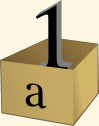
\includegraphics[width=1cm]{a1box.png}
  }
\end{textblock}

\begin{textblock}{5}(6,6.8)
  \visible<2->{
    
\includegraphics[width=1.1cm]{a1tag.png}
  }
\end{textblock}

\begin{textblock}{5}(6.8,10)
  \visible<3->{
    
\includegraphics[width=0.45cm]{1.png}
  }
\end{textblock}

\begin{textblock}{5}(8,10)
  \visible<3->{
    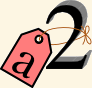
\includegraphics[width=1cm]{a2tag.png}
  }
\end{textblock}

\begin{textblock}{5}(6.8,12.8)
  \visible<4->{
    
\includegraphics[width=0.45cm]{1.png}
  }
\end{textblock}

\begin{textblock}{5}(8,12.8)
  \visible<4->{
    
\includegraphics[width=1.8cm]{ab2tag.png}
  }
\end{textblock}

\end{frame}

% -----------------------------------------------
\begin{frame}[fragile]
\frametitle{Numbers}
\begin{itemize}
\item Integers
\begin{lstlisting}
x = 0
age = 20 
size_of_household = 5

print type(age)
# <type 'int'>

# can handle arbitrarily large numbers
huge = 10 ** 100 + 1
\end{lstlisting} 

\item Floating-point Numbers
\begin{lstlisting}
g = 0.1
f = 6.67384

velocity = 1.  # it is the dot (.) that makes it a float
print velocity
# 1.0
type(velocity)
# <type 'float'>
\end{lstlisting}
\end{itemize}
\end{frame}

% -----------------------------------------------
\begin{frame}[fragile]
\frametitle{Numeric Expressions}
\begin{itemize}
\item Most of the arithmetic operators behave as expected.
\begin{lstlisting}[escapechar=\%]
a = 10
b = 20
print a %\--% (b ** 2) + 23 
# -367

x = 2.0
print x / 0.1
# 20.0
\end{lstlisting}
\item Watch out for integer divisions. In Python 2, it
      \emph{truncates down} to an integer.
\begin{lstlisting}[escapechar=\%]
print 10 / 3
# 3 (in Python 2)\hspace{1cm}3.3333333333333335 (in Python 3)
print %\--%10 / 3
# -4 (in Python 2)\hspace{1cm}-3.3333333333333335 (in Python 3)

# a solution: use floating point numbers
print 10.0 / 3.0
# 3.3333333333333335 (in both Python 2 and 3)   
\end{lstlisting}
\end{itemize}
\end{frame}

% -----------------------------------------------
\begin{frame}[fragile]
\frametitle{Quiz}
\begin{itemize}
\item What is the remainder of 5 divided by 2?
\item An answer:
\begin{lstlisting}[escapechar=\%]
# an answer
dividend = 5
divisor = 2

quotient = dividend // divisor
remainder = dividend - (quotient * divisor)
print "remainder:", remainder

# another answer
print "remainder:", dividend % divisor
\end{lstlisting}
\item What is the remainder of 2837465 divided by 2834?
\item An answer using the modulus operator (\%):
\begin{lstlisting}
print 2837465 % 2834
\end{lstlisting}
\end{itemize}
\end{frame}

% -----------------------------------------------
\begin{frame}[fragile]
\frametitle{String Literals}
\begin{itemize}
\item A string is a sequence of characters.
\begin{lstlisting}[escapechar=\%]
# either double (") or single(') quotes for creating string literals.
name = "Changarilla"
file_name = 'workshop.tex'

# triple-quoted string
starwars = %{\color{string}"""}%
%{\color{string}A long time ago is a galaxy far, far away...}%

%{\color{string}It is a period of civil war. Rebel}%
%{\color{string}spaceships, striking from a hidden}%
%{\color{string}base, have won their first victory}%
%{\color{string}...}%

%{\color{string}What is the last character of this string?}%
%{\color{string}"""}%

last_char = starwars[%\--1%]
print ord(last_char), ord("\n")
# 10 10
\end{lstlisting}
\end{itemize}
\end{frame}

% -----------------------------------------------
\begin{frame}[fragile]
\frametitle{Working with strings}
\begin{itemize}
\item Strings are immutable.
\begin{lstlisting}
s = "abcde"
s[0] = "x" # trying to change the first char to "x"
# TypeError: 'str' object does not support item assignment

t = "x" + s[1:] # creating a new string
print t
# xbcde
\end{lstlisting} 
\item Many functions and methods are available. 
\begin{lstlisting}
s = "abcde"
print s + s # concatenation 
# abcdeabcde

print len(s)
# 5

print s.find("c") # index is 0-based. returns -1 if not found
# 2
\end{lstlisting} 
\end{itemize}
\end{frame}

% -----------------------------------------------
\begin{frame}[fragile]
\frametitle{String Manipulation}
\begin{itemize}
\item<1-> A few more string methods.
\begin{lstlisting}
s = "abcde"
print s.upper(), "XYZ".lower()
# ABCDE, xyz

print "   xxx  yy  ".strip()
# xxx yy

print "a,bb,ccc".split(",")
# ['a', 'bb', 'ccc']
\end{lstlisting}
\item<2-> What are "methods"?
\begin{itemize}
\item<3-> Functions which are a member of a type (or class).
\item<4-> \lstinline{int}, \lstinline{str}, \lstinline{Word Document}
          are types (or classes).
\item<4-> \lstinline{2}, \lstinline{"abcde"}, \lstinline{diary.docx}
          are an \emph{instance} (or \emph{object}) of the
          respective type.
\item<4-> Types have members: properties (data) and methods (functions).
\end{itemize}
\end{itemize}

\begin{textblock}{5}(9,3.6)
  \visible<4->{
    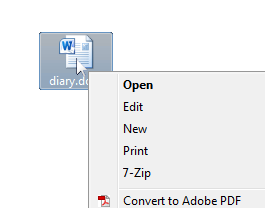
\includegraphics[width=4cm]{methods.png}
  }
\end{textblock}

\end{frame}

% -----------------------------------------------
\begin{frame}[fragile]
\frametitle{Two Ways to Format}
\begin{itemize}
\item \lstinline{format()} method.
\begin{lstlisting}
print "The answer is {0}".format(21)
# The answer is 21
print "The real answer is {0:6.4f}".format(21.2345678)
# The answer is 21.2346
\end{lstlisting}
\item Formatting operator.
\begin{lstlisting}
print "The answer is %d" % 21
# The answer is 21
print "The real answer is %6.4f" % 21.2345678
# The answer is 21.2346
\end{lstlisting}
\end{itemize}
\end{frame}

% -----------------------------------------------
\begin{frame}[fragile]
\frametitle{Quiz}
\begin{itemize}
\item Say hello to Simba and friends. Use print statement(s).
    The output should look like below. (Hint: Use
    \{0:s\} or \%s for the place holder.)
\begin{lstlisting}
Hello, Simba!
Hello, Timon!
Hello, Pumbaa!
\end{lstlisting}
\item An answer:
\begin{lstlisting}
friends = ["Simba", "Timon", "Pumbaa"]
hello_template = "Hello, %s!"

for friend in friends:
    print hello_template % friend
\end{lstlisting}
\end{itemize}
\end{frame}

% -----------------------------------------------
\begin{frame}[fragile]
\frametitle{Raw Strings}
\begin{itemize}
\item Within a string literal, escape sequences start
      with a backslash (\textbackslash)
\begin{lstlisting}
a_string = 'It\'s a great day\nto learn \\Python\\.\n 1\t 2\t 3'
print a_string
# It's a great day
# to learn \textbackslash{}Python\textbackslash{}.
# 1\hspace{1cm}2\hspace{1cm}3
\end{lstlisting}

\item A \emph{raw} string literal starts with the prefix
      \lstinline{r}. In a raw string, the backslash
      (\textbackslash) is not special.
\begin{lstlisting}[escapechar=\%]
import re

# raw strings are great for writing regular expression patterns.
p = re.compile(%{\color{string}r}%"\d\d\d-\d\d\d\d")
m = p.match('123-4567')
if m is not None:
    print m.group()
# 123-4567
\end{lstlisting}
\end{itemize}
\end{frame}
 
% -----------------------------------------------
\begin{frame}[fragile]
\frametitle{Unicode Strings}
\begin{itemize}
\item<1-> You can create Unicode strings using the \lstinline{u} prefix
      and "\textbackslash{}u" escape sequences. 
\begin{lstlisting}[escapechar=\%]
a_string = %{\color{string}u}%"Euro \u20AC" # \textbackslash{}u followed by 16-bit hex value xxxx
print a_string, len(a_string)
# Euro \euro{} 6
\end{lstlisting}
\item<2-> Unicode strings are sequences of \emph{code points}.
\item<2-> Code points are numbers, each representing a ``character''.
      e.g., U+0061 is `Latin small letter a'.
\item<2-> Unicode text strings are \emph{encoded} into
      bytes. UTF-8 is one of many Unicode encodings,
      using one to four bytes to store a Unicode ``character''.
\item<2-> Once you have Unicode strings in Python,
      all the string functions and properties work as expected.
\end{itemize}
\end{frame}
 
% -----------------------------------------------
\begin{frame}[fragile]
\frametitle{Best Practices According to 
            Thomas Wouters\cite{Wouters2012}}
\begin{itemize}
\item Never mix unicode and bytecode [i.e. ordinary] strings.
\item Decode bytecode strings on input.
\item Encode unicode strings on output.
\item Try automatic conversion (\lstinline{codecs.open()})
\item Pay attention to exceptions, \lstinline{UnicodeDecodeError}
\item An example
\begin{lstlisting}[escapechar=\%]
ustr = %{\color{string}u}%"Euro \u20AC"  # Euro \euro{}

# Python's default encoding codec is 'ascii'
ustr.encode()
# UnicodeEncodeError: 'ascii' codec can't encode characater  'u\textbackslash{}u20ac' 
utf_8 = ustr.encode("UTF-8") # encoding to UTF-8 works fine
# this takes 8 bytes. five one-byte's and one three-byte

# now we want to decode to ascii, ignoring non-ascii chars
print utf_8.decode("ascii", "ignore")
# Euro  (no euro symbol character)
\end{lstlisting}
\end{itemize}
\end{frame}

% -----------------------------------------------
\begin{frame}[fragile]
\frametitle{None}
\begin{itemize}
\item Is a place-holder, like NULL in other languages.
\begin{lstlisting}
x = None
\end{lstlisting}
\item Is a universal object, i.e., there is only one None.
\begin{lstlisting}
print None is None
# True
\end{lstlisting}
\item Is evaluated as False.
\begin{lstlisting}
x = None
if x:
    print "this will never print"
\end{lstlisting}
\item Is, however, distinct from others which are False.
\begin{lstlisting}
print None is 0, None is False, None is []
# False, False, False
\end{lstlisting}
\end{itemize}
\end{frame}

% -----------------------------------------------
\begin{frame}[fragile]
\frametitle{Core Data Types}
\begin{itemize}
\item Basic core data types: int, float, and str.
\item "Python is dynamically, but \emph{strongly} typed."
\begin{lstlisting}
n = 1.0
print n + "99"
# TypeError: unsupported operand types(s) for +: 'int' and 'str'
\end{lstlisting}
\item Use \lstinline{int()} or \lstinline{float()}
      to go from str to numeric
\begin{lstlisting}
print n + float("99")
# 100.0
\end{lstlisting}
\item \lstinline{str()} returns the string representation
      of the given object.
\begin{lstlisting}
n = 1.0
print str(n) + "99"
# 1.099 
\end{lstlisting}
\end{itemize} 
\end{frame}

% -----------------------------------------------
\begin{frame}[fragile]
\frametitle{Operators}
\begin{itemize}
%\item In an expression, \lstinline{3 + 4}, the
%      symbol \lstinline{+} is an addition operator;
%      \lstinline{3} and \lstinline{4} are called operands.
\item Python supports following types of operators:

\begin{itemize}
\item Arithmetic (\lstinline{+  -  *  /  %  **  //})
\item Comparison (\lstinline{==  !=  >  <  >=  <=})
\item Assignment (\lstinline{=  +=  -=  *=  /=  %=  **=  //=})
\item Logical (\lstinline{and or not})
\item Bitwise (\lstinline{&  |  ^  ~  <<  >>})
\item Membership (\lstinline{in  not in})
\item Identity (\lstinline{is  is not})
\end{itemize}
\end{itemize}
%\note{An expression is something that is evaluated into
%      a value.}
%\note{An operator is a language construct that
%      in general behaves like a function, but
%      is syntactically and semantically different
%      from a function. For instance, it works on
%      operands and does not accepts arguments.}
%\note{arithmetic operator, \lstinline{%} is a modulus
%      operator, dividing left hand operand by right hand
%      operand and returns remainder.}
%\note{arithmetic operator, \lstinline{//} is called 
%      floor division operator, returning the largest integer
%      that is smaller than or equal to the quotient.}
\end{frame}

% -----------------------------------------------
\begin{frame}[fragile]
\frametitle{A Few Surprises}
\begin{itemize}
\item Power operator (\lstinline{**}) binds more tightly
      than unary operators on the left.
\begin{lstlisting}[escapechar=\%]
a = %\--%2**2
print a
# -4
# solution: parenthesize the base
print (%\--%2)**2
# 4 
\end{lstlisting}
\item Comparisons can be chained. 
\begin{lstlisting}
x < y <= z         # y is evaluated only once here
\end{lstlisting}
is equivalent to
\begin{lstlisting}
x < y and y <= z
\end{lstlisting}
\item Logical operators (\lstinline{and}, \lstinline{or})
      short-circuit evaluation and return 
      an \emph{operand}.
\begin{lstlisting}
print 3 or 2
# 3
\end{lstlisting}
\end{itemize}
\end{frame}

% -----------------------------------------------
\begin{frame}[fragile]
\frametitle{Quiz}
\begin{itemize}
\item Demographic and Health Surveys (DHS) Century
Month Code (CMC)\cite[p.5]{MEASUREDHSPlus} provides an easy way
working with year and month.
\\~\\
The CMC is
an integer representing a month, taking
the value of 1 in January 1900, 2 in
February 1900, \ldots, 13 in January 1901, etc.
The CMC in February 2011 is 1334.
\\~\\
What is the CMC for this month, i.e., January, 2014?
\item<2-> An answer:
\begin{lstlisting}[escapechar=\%]
month = 5
year = 2015
cmc = 12 * (year %\--% 1900) + month
print cmc for year(%\%%d) month(%\%%d) is: %\%%d" %\%% (year, month, cmc)
%\#% cmc for year(2015) month(5) is: 1385
\end{lstlisting}
\item<3-> What is the month (and year) of CMC 1000? 
\begin{lstlisting}[escapechar=\%]
print "cmc(%\%%d) is year(%\%%d) and month(%\%%d)" %\%% (1000,
    (1900 + (1000 // 12)), (1000 %\%% 12))
\end{lstlisting}
\end{itemize}
\end{frame}

% -----------------------------------------------
\begin{frame}[fragile]
\frametitle{Quiz}
\begin{itemize}
\item According to U.S. National Debt Clock,
      the outstanding public debt, as of 
      a day in 2012, was a big number:
\begin{lstlisting}
debt = 17234623718339.96
\end{lstlisting}
      Count how many times the digit 3 appears
      in the number.

      (Hint: create a string variable and use
       the \lstinline{count()} method of
       the string type.)  
\item<2-> An answer:
\begin{lstlisting}
sdebt = "17234623718339.96"
print sdebt.count("3")
# 4
\end{lstlisting}
\item<3-> (tricky) It feels rather silly to rewrite the
          value as a string.
          Can you think of a way to \emph{convert}
          the number into a string? 
\item<3-> An answer:
\begin{lstlisting}
print "{0:17.2f}".format(debt).count("3")
# 4
\end{lstlisting}
\end{itemize}
\end{frame}

% -----------------------------------------------
\begin{frame}[fragile]
\frametitle{Flow Control}
\begin{itemize}
\item Conditional Execution (\lstinline{if})
\item Iteration
\begin{itemize}
\item \lstinline{while} loop
\item \lstinline{for} loop
\end{itemize}
\end{itemize}
\end{frame}

% -----------------------------------------------
\begin{frame}[fragile]
\frametitle{IF}
\begin{itemize}
\item IF statement is used for conditional execution.
\begin{lstlisting}
if x > 0:
    print "x is positive"
else:
    print "x is zero or negative" 
\end{lstlisting}
\item Only one suite (block of statements) under a
      \lstinline{True} conditional expression is executed.
\begin{lstlisting}
me = "rock"
wins = 0

if you == "paper":
    print "You win!"
elif you == "scissors":
    print "I win!"
    wins += 1
else:
    print "draw"      
\end{lstlisting}
\end{itemize}
\end{frame}

% -----------------------------------------------
\begin{frame}[fragile]
\frametitle{Compound statements}
\begin{itemize}
\item \lstinline{if}, \lstinline{while}, and \lstinline{for}
      are \emph{compound} statements, which have
      one or more \emph{clauses}. A \emph{clause}, in turn,
      consists of a \emph{header}
      that ends with a colon (\lstinline{:}) and 
      a \emph{suite}.
\item A suite, a block of statements, is identified by \emph{indentation}.
\begin{lstlisting}
a = 1
if a > 0:
    desc = "a is positive"       # these two lines form a suite 
    print a, desc                #
                                 # (blank line ignored)
print "done"                     # This line being started "dedented"
                                 # signals the end of the block

    if a > 0:                    # indentation error
desc = "a is positive"           # indentation error

if a > 0:                        # OK
          desc = "a is positive" # OK
          print a, desc          # OK
else:                            # OK 
     print a                     # OK
\end{lstlisting}
\end{itemize}
\end{frame}

% -----------------------------------------------
\begin{frame}[fragile]
\frametitle{Compound statements}
\begin{itemize}
\item The amount of indentation does not matter (as long
      as the same within a level). Four
      spaces (per level) and no tabs are the convention.
\item Use editor's python mode, which prevents/converts
      <TAB> to (four) spaces.
\item Why indentation? A good answer at:
      \url{http://tinyurl.com/kxv9vts}.
\item For an empty suite, use \lstinline{pass} statement,
      which does nothing.
\end{itemize}
\end{frame}

% -----------------------------------------------
\begin{frame}[fragile]
\frametitle{Quiz}
\begin{itemize}
\item Given an integer n, print out "Even" if n is an
    even number or "Odd" if n is an odd number. (Hint:
    (n \% 2 == 0) is true when n is an even number.
\item An answer:
\begin{lstlisting}[escapechar=\%]
n = 3
if (n %\%% 2 == 0):
    print "Even"
else:
    print "Odd"
\end{lstlisting}
\item Given an integer n, print out "Even" if n is an
    even number except zero or "Odd" if n is an odd number.
    When n is equal to zero (0), then print out "Even and zero",
    instead of just "Even".
\item An answer:
\begin{lstlisting}[escapechar=\%]
n = 3  # using the if else expressions, not if else statements
print ("Odd" if (n%\%% 2) else "Even") + ("" if n else " and zero")
\end{lstlisting}
\end{itemize}
\end{frame}

% -----------------------------------------------
\begin{frame}[fragile]
\frametitle{WHILE}
\begin{itemize}
\item Repeats a block of statements
      as long as the condition remains \lstinline{True}.
\begin{lstlisting}
total = 0
n = 0
while n < 10:
    print n, total
    n += 1
    total += n
# 0 0
# 1 1
# 2 3
# ...
# 9 45
\end{lstlisting}
\item \lstinline{break} terminates the loop
      immediately.
\item \lstinline{continue} skips the remainder
      of the block and goes back to the test 
      condition at the top.
\end{itemize}
\end{frame}

% -----------------------------------------------
\begin{frame}[fragile]
\frametitle{FOR}
\begin{itemize}
\item \lstinline{for} is used to iterate over a
      sequence.
\begin{lstlisting}
days = ["Sunday", "Monday", "Tuesday", "Wednesday",
        "Thursday", "Friday", "Saturday"]

for day in days:
    if day == "Friday":
        print "I am outta here."
        break
    print "Happy" + " " + day + "!"

# Happy Sunday!
# Happy Monday!
# ...
# Happy Thusday!
# I am outta here.
\end{lstlisting}
\end{itemize}
\end{frame}

% -----------------------------------------------
\begin{frame}[fragile]
\frametitle{FOR}
\begin{itemize}
\item Another example.
\begin{lstlisting}
numbers = range(5)
print numbers
# [0, 1, 2, 3, 4]

for n in numbers:
    print n,
    if n % 2 == 0:
         print "is even"
    else:
         print "is odd" 

# 0 is even
# 1 is odd
# 2 is even
# 3 is odd
# 4 is even      
\end{lstlisting}
\end{itemize}
\end{frame}

% -----------------------------------------------
\begin{frame}[fragile]
\frametitle{Quiz}
\begin{itemize}
\item Write either a while or a for loop to add integers from 1 to
    a given positive integer, n (n >= 1). For example, when n is 3,
    your program should print out 6, when n is 10, 55.
    (Hint: It is easy to get an infinite loop. If you don't see
    output and kernel keeps running (indicated by the filled circle
    under the Python logo on the top right corner of ipython notebook),
    then interrupt the kernel by clicking on the ipython notebook
    menu, Kernel > Interrupt, and fix the error.)
\item An answer:
\begin{lstlisting}[escapechar=\%]
n = 3
i = 1
total = 0
while (i <= n):
   total = total + i
   i = i + 1
print total
\end{lstlisting}
\end{itemize}
\end{frame}


% -----------------------------------------------
\begin{frame}[fragile]
\frametitle{Quiz}
\begin{itemize}
\item You may have noticed that it is rather silly to use a loop
    to calculate this sum. Calculate the sum of integers from 1
    to n (n >= 1) directly without a loop. (Hint the sum is also
    known as the "triangular number".)
\item An answer:
\begin{lstlisting}[escapechar=\%]
n = 3
print (n * (n + 1)) / 2
\end{lstlisting}
\end{itemize}
\end{frame}

% -----------------------------------------------
\begin{frame}[fragile]
\frametitle{File I/O}
\begin{itemize}
\item The built-in function, \lstinline{open()},
      returns a \lstinline{file} type object,
      unless there is an error opening the file.
\begin{lstlisting}
in_file = open("yourfile.txt", "r") # for reading
out_file = open("myfile.txt", "w") # for writing
\end{lstlisting}
\item Once we get the \lstinline{file} type object,
      then use its methods.
\begin{lstlisting}
# read all the contents from the input file
content = in_file.read()

# write out a line to the output file
out_file.write("hello?\n")

# close it when done
in_file.close()
out_file.close()
\end{lstlisting}
\end{itemize}
\end{frame}

% -----------------------------------------------
\begin{frame}[fragile]
\frametitle{Reading a file one line at a time}
\begin{itemize}
\item \lstinline{with} ensures that the file
      is closed when done.
\begin{lstlisting}
with open("lorem.txt", "r") as f: 
    for line in f:
        print line
\end{lstlisting}
\item Another example.
\begin{lstlisting}
# creating a file and writing three lines
with open("small.txt", "w") as f:
    f.write("first\n")
    f.write("second\n")
    f.write("third")

with open("small.txt", "r") as f:
    for line in f: 
        print line   # line includes the newline char  
# first    
#
# second
#
# third
\end{lstlisting}
\end{itemize}
\end{frame}

% -----------------------------------------------
\begin{frame}[fragile]
\frametitle{Defining and Calling a Function}
\begin{itemize}
\item Defined with \lstinline{def} and
      called by name followed by \lstinline{()}.
\begin{lstlisting}
def the_answer():
    return 42

print the_answer()
# 42
\end{lstlisting}
\item Argument(s) can be passed. 
\begin{lstlisting}
def shout(what):
    print what.upper() + "!"

shout("hello")
# HELLO!
\end{lstlisting}
\item If the function \lstinline{return}s nothing,
      then it returns \lstinline{None}.
\begin{lstlisting}
r = shout("hi")
# HI!
print r
# None
\end{lstlisting}
\end{itemize}
\end{frame}

% -----------------------------------------------
\begin{frame}[fragile]
\frametitle{Another example}
\begin{itemize}
\item CMC again
\begin{lstlisting}[escapechar=\%]
def cmc(year, month):
    ''' returns DHS Century Month Code ''' # doc string
    if year < 1900 or year > 2099:
        print "year out of range"
        return
    if month < 1 or month > 12:
        print "month out of range"
        return
    value = (year %\--% 1900) * 12 + month
    return value

print cmc(2014, 1)
# 1369
print cmc(2014, 15)
# month out of range
# None               
\end{lstlisting}
\end{itemize}
\end{frame}

% -----------------------------------------------
\begin{frame}[fragile]
\frametitle{Quiz}
\begin{itemize}
\item Write a function odd(n) which returns true if given the
    number is odd or false otherwise. (Hint: Recall the remainder
    operator \%.)
\begin{lstlisting}[escapechar=\%]
def odd(n):
   return (n % 2 == 0)
\end{lstlisting}
\item Write a function, triangular(n), which returns the 
    triangular number n, that is the sum of integers from
    1 to the given number, n. For example, triangular(3)
    should return 6 and triangular(10) should return 55.
\begin{lstlisting}[escapechar=\%]
def triangular(n):
   return (n * (n + 1)) / 2
\end{lstlisting}
\item Print out the first 20 odd triangular numbers.
    (Hint: OEIS A014493)
\begin{lstlisting}[escapechar=\%]
for i in range(1, 21):
   print triangular(i),
\end{lstlisting}
\end{itemize}
\end{frame}

% -----------------------------------------------
\begin{frame}[fragile]
\frametitle{Local and Global Variables}
\begin{itemize}
\item Within your function:
\begin{itemize}
\item A new variable 
      is \emph{local}, and independent of the global
      var with the same name, if any.
\begin{lstlisting}
x = 1                    # global (or module)

def my_func():
    x = 2                # local 
my_func()                
print x                  # 1
\end{lstlisting}
\item Both local and global variables can be read.
\item Global variables can be writen to once \emph{declared} so.
\begin{lstlisting}
x = 1                    

def my_func():
    global x
    x = 2                # global 
my_func()                
print x                  # 2
\end{lstlisting}
\end{itemize}
\end{itemize}
\end{frame}

% -----------------------------------------------
\begin{frame}[fragile]
\frametitle{Quiz}
\begin{itemize}
\item Write a function that returns Body Mass Index
      (BMI)
      of an adult given weight in kilograms and 
      height in meters.
      (Hint: BMI = weight(kg) / (height(m) squared).

      For instance, if a person is 70kg and 1.80m,
      then BMI is about 21.6.)

\item<2-> An answer.
\begin{lstlisting}
def bmi(kg, m):
    return float(kg) / (m ** 2)
\end{lstlisting}
\item<3-> Re-write
    the bmi function so that it accepts height in feet
    and inches, and the weight in pounds. (Hint. Make pound, foot,
    and inch arguments. Convert them into local
    variables, kg and m, before calculating bmi to return.)
\begin{lstlisting}
def bmi(foot, inch, pound):
    kg = 0.453592 * pound
    m = 0.0254 * (12 * foot + inch)
    return kg / (m ** 2)
\end{lstlisting}
\end{itemize}
\end{frame}

% -----------------------------------------------
\begin{frame}[fragile]
\frametitle{Importing a module}
\begin{itemize}
\item \lstinline{import} reads in a module, runs
      it (top-to-bottom) to create the module
      object.
\item Via the module object, you get access to its
      variables, functions, classes, \ldots
\item We've already seen an example of importing
      a standard regular expression module:
\begin{lstlisting}[escapechar=\%]
import re 

# compile() is a function defined within the imported re module.

p = re.compile(%{\color{string}r}%"\d\d\d-\d\d\d\d")
m = p.match('123-4567')
if m is not None:
    print m.group()
# 123-4567
\end{lstlisting}
\end{itemize}
\end{frame}

% -----------------------------------------------
\begin{frame}[fragile]
\frametitle{Another example}
\begin{itemize}
\item There are many standard modules that come
      already installed, and be ready to be imported.
\begin{lstlisting}[escapechar=\%]
import math

s = math.sqrt(4.0)
print "4.0 squared is {0:.2f}".format(s)
# 4.0 squared is 2.00
\end{lstlisting}
\item You can selectively import as well.
\begin{lstlisting}
from math import sqrt # import sqrt() alone

print sqrt(9.0)       # no "math."
# 3.0
\end{lstlisting}
\item You can import your own Python script file (.py)
      the same way. The default import path includes
      the current working directory and its sub-directories.
\begin{lstlisting}
import hello   # suppose that hello.py defines a main() function

hello.main()
# "hello, World!"
\end{lstlisting}
\end{itemize}
\end{frame}

% -----------------------------------------------
\begin{frame}[fragile]
\frametitle{Quiz}
\begin{itemize}
\item Write a function such that, given a BMI value, 
    returns the BMI category as a string. Recall the
    categories are:
{\tiny
\begin{table}[h]
\begin{tabular}{r l}
Underweight & less than 18.5 \\ 
Normal weight & 18.5 upto but not including 25 \\
Overweight & 25 upto but not including 30 \\
Obesity & 30 or greater \\
\end{tabular}
\end{table}
}
For instance, the function should return a string 
"Normal weight", when it is called with an argument
of, say 20. (Hint: use conditional statements 
i.e., \lstinline{if ... elif ...})
\begin{lstlisting}
def bmi_category(bmi):
    if bmi < 18.5:
        return "Underweight"
    elif bmi < 25.0:
        return "Normal weight"
    elif bmi < 30.0:
        return "Overweight"
    else:
        return "Obesity"
\end{lstlisting} 
\end{itemize}
\end{frame}

% -----------------------------------------------
\begin{frame}[fragile]
\frametitle{Quiz}
\begin{itemize}
\item Print out a BMI table showing several lines of
    a pair: a BMI value and its category. BMI value
    may start at 15 and go up by 3 up to 36.
    (Hint: use a loop)
\begin{lstlisting}
for bmi in rnage(15, 36 + 1, 3):
    print "\%3.0f \%s" \% (bmi, bmi_category(bmi))
\end{lstlisting}
\end{itemize}
\end{frame}

% -----------------------------------------------
\begin{frame}[fragile]
\frametitle{Quiz (cont.)}
\begin{itemize}
\item Create a comma-separated values (.csv) file
    of the BMI table. (Hint: You may start with below,
    and modify it as neccessary.) 
\begin{lstlisting}
import csv

with open("test.csv", "wb") as f:
    my_writer = csv.writer(f)
    bmi = 15
    while bmi < 36:
        cat = bmi_category(bmi)
        my_writer.writerow([bmi, cat])
        bmi += 3
\end{lstlisting}
\end{itemize}

\begin{textblock}{5}(11.5,9.5)
  \visible<1->{
    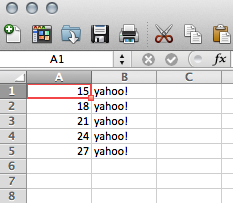
\includegraphics[width=3cm]{testcsv.png}
  }
\end{textblock}

\end{frame}

% -----------------------------------------------
\begin{frame}[fragile]
\frametitle{Summary}
\begin{itemize}
\item Using Python interactively or by running a script.
\item Comments.
\item Variables and assignment semantics.
\item Core data types (int, float, str, None).
\item Operators.
\item Conditionals and Looping.
\item Defining and using functions.
\item Basic File I/O.
\item Importing a module.
\end{itemize}
\end{frame}

% -----------------------------------------------
\begin{frame}%[allowframebreaks]
  \frametitle{References}
  \bibliographystyle{acm}
  \scriptsize
  \bibliography{references}
\end{frame}

\end{document}
